%%% Local Variables:
%%% mode: latex
%%% TeX-master: "../report"
%%% End:

It is not only for stack or heap elements which we need to store information
about their type. Sub-routines and object fields also has type information which
we need to keep track of, but the information is not the same. For instance, a
stack or heap element has types describing the type of its value. A sub-routing
will need have a type signature, describing the types of it's parameters, a name
and possible properties. Similarly an object field will have (TODO).

Therefore, we need to abstract our type information a level higher, letting us
better describe different types of types. Instead of storing the different data
different places, we will have a centralized table, containing all meta
information. This will be named the \term{meta table} and will need to be
dynamically sized to support reflection and generating new types at run-time.

All meta objects in the machine will have a tag defining which of type of
information it contains.
\begin{ccode}
enum meta_tag_e {
    TYPE,
    METADATA,
    FIELD,
};
typedef enum meta_tag_e meta_tag;

struct meta_base_s {
    meta_tag tag;
};
typedef struct meta_base_s meta;

struct meta_type_s {
    meta base;

    type *type;
};
typedef struct meta_type_s meta_type;
\end{ccode}
In the case of {\tt TYPE} it will be cast to the {\tt meta\_type} which allows
access to the {\tt type} referenced described below.

We will describe each type of meta information in turn.

\subsubsection{Types}
The executable file, containing the program to be run, declares a type table for
the custom types created by the program. Through out the executable, these types
are referenced through the type's index in this table. This table is static, so
the machine can analyze how many types it contains. The types will be parsed
from the executable and added to the global meta table lazily. This reduces
the initial overhead of parsing the executable.

The machines built-in types are described by a type tag, implemented as an enum:
\begin{ccode}
enum type_tag_e {
    ACTIVATION_ELEMENT = 0,
    ANY                = 1,
    BOOL               = 2,
    INT8               = 3,
    UINT8              = 4,
    ...
};
typedef enum type_tag_e type_tag;
\end{ccode}
The enums integer value is used to describe its index in the meta table. There
will always only be {\it one} instance of each type, so two equal types can
never be referenced by two different pointers. This invariant lets the machine
check type equality through comparing the type pointers.

More specifically, all types in the machine is stored internally through
structs. Simple types implement the {\tt type\_base} struct, which is extended
in composite types. For instance, a reference is represented as:
\begin{ccode}
struct type_base_s {
    type_tag tag;
    int size;
};
typedef struct type_base_s type;

struct type_ref_s {
    type base;
    type *ref_type;
};
typedef struct type_ref_s type_ref;
\end{ccode}

All types are always passed around in the machine through the {\tt type}
name. If the type is for instance a reference, i.e. implementing the {\tt
  type\_ref}, it is cast so its reference specific attributes can be
referenced. The type of type is checked through the tag, defined in {\tt
  type\_base}. Another important entry in the type structure is the size
attribute. This is essential, as it tells the machine how much memory is needed
to store its value on either the stack or heap.

Types from the executable are mapped from its index in the binary type table to
the machines meta table. The types from the binary file is parsed lazily,
i.e. the first time the program tries to look-up a type through its index in the
binary type table, it is parsed and stored in the machine's type table. This is
done in the virtual machine implementation's {\tt vm\_lookup\_elf\_type}
function, which takes a reference to the type table and a type index in the
binary file.

TODO: update look-up shit
To get a reference to a built-in type, one can look-it up through a look-up
function, which takes the name of the built-in type and the type table:
\begin{ccode} % TODO: update
type *lookup_type(type **ttable, type_tag tag)
{
    int i;
    for (i = 0; i < ttable_size; i++) {
        if (ttable[i] == NULL)
            continue;

        if (ttable[i]->tag == tag)
            return ttable[i];
    }

    log_errf(TYPE_ERROR, "could not find type with tag %d", tag);

    return NULL;
}
\end{ccode}
The function iterates the types in the type table, matching on its tag. The null
check is used to avoid types from the binary file not yet parsed, to be skipped.

Currently, if a type is not found, an error is thrown, halting the machine (TODO
exceptions).

When trying to box a stack element trough the {\tt box} instruction, the top
element is popped off the stack and stored on the heap. An element with a
reference to the heap object is in turn pushed to the stack. The type of the new
element will be a {\tt Reference<t>} type, where {\tt t} is the type of the
stack element which was boxed. If this type is not found in the type table
already it will have to be generated. This is done by TODO.

Composite types are made through (TODO).

Most types can be converted, with some exceptions (TODO signature type). If a
value is converted to a type with smaller size, for instance an {\tt Int32} to
{\tt Int8}, the value is truncated (TODO exception)?

All types are garbage collected. This means, when a type is no longer used by
the program, it's memory is freed. (TODO)

% floats

When handling floating point precision numbers we will, as aforementioned, use
the IEEE 754 standard~\cite{ieee754}. This is a technical standard defining the
arithmetic format, i.e. the finite range and special values, rounding rules,
operations, exception handling and interchange formats. Its values include
finite numbers (within a certain maximum or minimum, depending on the size), two
infinities (plus and minus) and a NaN (not a number).

A floating point number is always represented by a sign, a fraction (also called
significant or mantissa), and an exponent. A can have multiple alternative
representations, for instance $1.10 \cdot 10^2$ can also be written as
$11.00 \cdot 10^1$. This though, should not have any effect on the result of
arithmetic operations. When storing the number in memory, one bit is used for
sign and the rest for exponent and fraction, depending on the size. The most
common the is single and double precision, which is respectively 4 and 8 bytes
in size. Their binary representation is called {\tt binary32} and {\tt
  binary64}.

\begin{figure}[H]
  \centering
  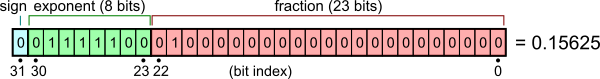
\includegraphics[scale=0.7]{images/ieee32.png}
  \caption[Caption for LOF]{IEEE-754 binary32 encoding~\footnotemark}
\end{figure}
\footnotetext{\url{https://en.wikipedia.org/wiki/Single-precision_floating-point_format}}

When parsing a {\tt binary32} we start by taking all the correct bits out into
separate numbers. We can then apply the following formula to get its decimal
value.

\begin{equation}
  value = (-1)^{sign} \cdot (1 + \sum^{23}_{i=1} b_{23-i}2^{-i}) \cdot 2^{e - 127}
\end{equation}

% type lattice

When performing arithmetic instruction on numbers, the type of the number has to
be taken into careful consideration. There is always the common pitfall of not
handling overflow of numbers, but also when doing arithmetic operations of two
different types of numbers. If a program, for instance, divides a floating point
precision number by an integer number, will the result be an floating point or
integer? Instead of having a long list of each case, the choice will be defined
by a type lattice. This type lattice will control what type the result is of a
given operation between two numbers of different types.

All binary arithmetic operations follow the same type lattice (TODO:
correct?). The type lattice has the following set of rules matching which
operand that is to be converted, where the resulting conversion is also the type
of the result.
\begin{itemize}
  \item If both operands is of the same type, nothing needs to be done.
  \item Otherwise, if either operand is a double floating-point precision number, the other
    operand is converted to a double also.
  \item Otherwise, if either operand is a single floating-point precision number, the other
    operand is converted to a float also.
  \item Otherwise, if either operand is of different signs, i.e. one is unsigned
    and the other is signed, the signed operand is converted to the an signed
    integer of the largest size of the two operands.
  \item Otherwise, the operands is of integer types of the same sign, where we
    return the largest of the two.
\end{itemize}

If none of the rules apply it will mean that at least one of the given operands
is of a type not supporting arithmetic operations. In this case, an exception
will be thrown.

If a type is converted to a type of smaller size, the value it truncated and
will have the chance of overflowing, changing the value of the number. The {\tt
  noOverflow} prefix defines if an exception should be thrown if overflow
occurs. There are though, separate instruction for saturated arithmetic
operations, where overflow is handled by saturating the number of the given
type. For instance, converting {\tt 0xFFFF} of type {\tt Int16} to {\tt Int8}
will become {\tt 0xFF}.
